\chapter{Cwm Taf data analysis}

\renewcommand{\texpath}{chapters/data/paper/tex}

In this chapter a summative and exploratory analysis of a patient-episode dataset
will be conducted. This dataset has been provided by the Cwm Taf University
Health Board and details the costs associated with treating patients during
their time in hospital. The focus of this analysis is to better understand and
observe variation in these costs; in particular, how a selection of
cost-related attributes are distributed across the entire dataset and how
they interact with one another. These attributes are comprised of non-trivial
cost components and a set of clinical attributes typically associated with
changes in costs. The ensuing analysis will show that while the bulk of the data
corresponds to short-stay and relatively low-impact spells of treatment, there
are long, heavy tails with high levels of variation in each of these variables.

Following this, a framework for the analysis of slices within the data is
established, using the diabetic population as an example. This framework
provides another dimension to the overall analysis through the use of comparison
and contrast but the intended impact is ultimately lost due, again, to high
levels of variation. Finally, the analysis looks toward other methods of
extracting intrinsic structures built within the data. These methods are
generally based in the clustering of patients and spells specifically, and so
the framework is still applicable. There is also discussion of the clustering of
patient pathways and how such analysis could highlight areas, procedures or
departments that influence variation, and those that leave well enough alone.


\section{An overview of the data}\label{sec:overview}
\graphicspath{{chapters/data/paper/img/external/}}

\subsection{Data structure}\label{subsec:structure}

Before any analysis can be conducted, it is best to learn how the data is
structured and how it has been prepared. This dataset is comprised of
approximately two and a half million episode records for patients from across
Wales that were treated in the Prince~Charles and Royal~Glamorgan hospitals
(South~Wales) from April 2012 through April 2017. An approximation for the
geographic distribution of patients is given in
Figure~\ref{fig:proportion_wales}.

\begin{figure}[htbp]
    \centering
    \includegraphics[width=\imgwidth]{proportion_wales.pdf}
    \caption{The proportion of total patients observed in the dataset by
    postcode district (e.g.\ CF24).}\label{fig:proportion_wales}
\end{figure}

An episode is defined to be any continuous period of care provided
by the same consultant in the same place. For instance, if a patient is admitted
to a general medical ward for diagnosis and testing, and then is referred to a
specialist consultant in oncology, then their first episode would end with their
testing, and a second episode of care would begin on the oncology ward. Each of
these episodes would correspond to a row in the dataset. If the patient was then
discharged, they would have completed a spell with two episodes.

In this analysis, looking at episode-level statistics will be avoided in favour
of a patient's spell-level statistics. Since the introduction of the `payment by
results' system for financial flows, it has been seen that focusing on the more
granular episode statistics can lead to the amount of resource or `activity'
consumed by a hospital to treat that patient being
overestimated~\cite{Aylin2004}.

Each episode is recorded as a row of roughly 260 attributes or columns,
including:

\begin{itemize}
    \item Personal information such as identification numbers, age, registered
        GP practice;
    \item Clinical quantities such as the number of diagnoses made and
        procedures conducted in that episode, admission and discharge dates and
        methods, and length of stay;
    \item A number of cost components which include the costs coming from
        various departments within the hospital, overall medical and ward costs,
        as well as overhead costs;
    \item Diagnosis (HRG, ICD-10) and procedure (OPCS-4) codes, as well as
        Charlson index scores for the appropriate chronic diseases.
\end{itemize}

Of the attributes listed here, the focus is on the total, net and summed
component costs, and a selection of other clinical variables \-- paying
particular attention to those attributes which are considered to be linked to an
overall contribution to the cost of care. Those attributes are: length of stay,
the maximum number of diagnoses during a spell, the total number of procedures
during a spell, and (separately) the number of spells associated with any given
patient.

\subsection{Cleaning the data}\label{subsec:formatting}

As with any real-world data analysis, a substantial amount of preprocessing and
formatting was required to make the data sufficiently consistent and suitable
for the intended purposes. This process included the removal of some superfluous
columns which added unwanted redundancy to the dataset, and a number of rows
that had been corrupted by some external storage software prior to this chapter's
beginning. In addition to this, some columns have been reformatted; namely those
whose entries were intended to be used as date-time objects later on. These
include admission and discharge dates, and financial bench periods.



As was discussed at the end of Section~\ref{subsec:structure}, the majority of
the attributes in the dataset will not be considered at this stage of the
analysis. This allows the focus to be on how the costs of care are distributed
and seen in the data. The subset of chosen attributes will frequently be
referred to as the set of `key attributes' but this choice of name does not
imply that the remaining attributes are not of interest or that they are in any
way unimportant.

The chosen, `key' attributes provide a base for understanding how the
costs and resources consumed by a patient in a spell are built up: cost
components give direct information on which departments and types of procedures
are being utilised; the length of stay can give an indication of the nature of
the spell and any default costs that may be incurred by spending more time in
hospital; and considering the maximum and total number of diagnoses and
procedures (respectively) in a spell allow for some insight into the severity or
complexity of a patient's spell in hospital.


\graphicspath{{chapters/data/paper/img/overview/}}
\subsection{Distributions and summative statistics}%
\label{subsec:distributions_statistics}

When looking at the distributions of the key attributes on the whole dataset,
displayed in Figures~\ref{fig:no_spells_bar}~\--~\ref{fig:netcost_kde}, it
is clear that the data is weighted towards low-cost, short-stay, and
otherwise low-impact patients. This behaviour is well-projected through
Figures~\ref{fig:no_spells_bar}~\&~\ref{fig:los_bar}. Here, it is clear that of
all the spells provided under the care of the health board that the majority are
day-cases, and that the patients being dealt with are one-time users of the
hospital system.

In general, the distributions themselves have long, pronounced tails. This
suggests that the effect of extreme cases, despite being a rarity, takes a toll
on the hospital system with respect to the cost of providing care.

\begin{figure}[htbp]
    \centering
    \includegraphics[width=\imgwidth]{no_spells_bar/main.pdf}
    \caption{Bar chart for the number of spells associated with a patient.}%
    \label{fig:no_spells_bar}
\end{figure}

\begin{figure}[htbp]
    \centering
    \includegraphics[width=\imgwidth]{los_bar/main.pdf}
    \caption{Bar chart for the total length of a spell, clipped at 21 days.
        \textit{Maximum 705 days.}}%
    \label{fig:los_bar}
\end{figure}

\begin{figure}[htbp]
    \centering
    \includegraphics[width=\imgwidth]{no_diag_bar/main.pdf}
    \caption{Bar chart for the maximum number of diagnoses in a spell.}%
    \label{fig:no_diag_bar}
\end{figure}

\begin{figure}[htbp]
    \centering
    \includegraphics[width=\imgwidth]{no_proc_bar/main.pdf}
    \caption{Bar chart for the total number of procedures in a spell.}%
    \label{fig:no_proc_bar}
\end{figure}

\begin{figure}[htbp]
    \centering
    \includegraphics[width=\imgwidth]{netcost_kde/main.pdf}
    \caption{Estimated probability density for the net cost of a spell, clipped
        at \pounds12,500. \textit{Maximum approx. \pounds369,000.}}%
    \label{fig:netcost_kde}
\end{figure}

Though the length and returning frequency of the spells are largely minimal and
tightly packed, their associated net costs are wildly variant. This is seen
immediately from inspecting Figure~\ref{fig:netcost_kde}. It would appear that
there is a distinct peak in the figure, but upon closer inspection of the scale
it becomes clear that this peak is little more than a blip; the most probable
net cost has a likelihood of less than one tenth of a percent. The remaining
values are distributed in a way that, given the scale, is near uniform, spanning
from approximately \pounds6000 up to \pounds369,000. A more detailed look at the
skeleton of this distribution, and those of the remaining key attributes, is
given in Table~\ref{tab:summative}.

\begin{table}[htbp]
    \resizebox{\linewidth}{!}{%
        \begin{tabular}{lrrrrrrrrrr}
\toprule
{} &       COST &       CRIT &      DRUG &      EMER &      ENDO &       HCD &       IMG &   IMG\_OTH &        MED &       NCI \\
\midrule
mean &    1834.93 &     -92.08 &     75.40 &      1.24 &     21.19 &     20.91 &     32.70 &     20.57 &     347.12 &    -30.92 \\
std  &    3771.16 &    1332.61 &    315.17 &     29.13 &     92.76 &    210.98 &    143.67 &    118.26 &     739.73 &     85.80 \\
min  &       4.50 & -250000.61 &     -0.57 &      0.00 &      0.00 &      0.00 &      0.00 &      0.00 &       0.00 & -12960.21 \\
25\%  &     347.67 &       0.00 &      7.18 &      0.00 &      0.00 &      0.00 &      0.00 &      0.00 &      44.45 &    -29.75 \\
50\%  &     749.49 &       0.00 &     20.00 &      0.00 &      0.00 &      0.23 &      0.08 &      0.00 &     130.67 &    -11.64 \\
75\%  &    1886.38 &       0.00 &     59.88 &      0.00 &      0.00 &      4.83 &     10.93 &      0.31 &     375.32 &     -3.02 \\
max  &  369168.93 &       0.00 &  63430.52 &  33347.89 &  11855.95 &  94411.85 &  46708.66 &  46708.66 &  116449.90 &      0.00 \\
\bottomrule
\end{tabular}

    }

    \resizebox{\imgwidth}{!}{%
        \begin{tabular}{lrrrrrrrrrr}
\toprule
{} &       NID &    NetCost &     OCLST &       OPTH &      OTH &  OTH\_OTH &      OUTP &        OVH &      PATH &  PATH\_OTH \\
\midrule
mean &     94.83 &    1742.85 &     13.30 &     160.11 &     1.37 &     0.97 &      0.57 &     354.82 &     36.20 &     23.29 \\
std  &    248.16 &    3185.31 &     58.74 &     486.24 &    11.67 &    10.15 &     26.79 &     734.05 &    135.47 &    122.71 \\
min  &      0.00 &       4.50 &      0.00 &       0.00 &     0.00 &     0.00 &      0.00 &       0.00 &      0.00 &      0.00 \\
25\%  &     14.99 &     347.32 &      0.00 &       0.00 &     0.00 &     0.00 &      0.00 &      84.86 &      0.00 &      0.00 \\
50\%  &     32.25 &     747.13 &      0.77 &       0.00 &     0.00 &     0.00 &      0.00 &     139.47 &      4.63 &      0.00 \\
75\%  &     83.36 &    1862.51 &      5.43 &       0.04 &     0.00 &     0.00 &      0.00 &     320.93 &     31.89 &     13.76 \\
max  &  84374.21 &  369168.93 &  12358.37 &  111396.20 &  1248.83 &  1248.83 &  10632.15 &  106428.61 &  70008.12 &  70008.12 \\
\bottomrule
\end{tabular}

    }

    \resizebox{\imgwidth}{!}{%
        \begin{tabular}{lrrrrrrrrrr}
\toprule
{} &  PATH\_OTH &      PHAR &  PROC\_NO &      PROS &   RADTH &     SECC &       SPS &       THER &  TRUE\_LOS &       WARD \\
\midrule
mean &     23.29 &     30.47 &     1.90 &     40.71 &    0.65 &     0.87 &     11.81 &      28.62 &      2.90 &     497.07 \\
std  &    122.71 &     86.70 &     2.21 &    343.57 &    8.01 &    27.43 &    149.46 &     181.58 &      9.21 &    1236.63 \\
min  &      0.00 &      0.00 &     0.00 &      0.00 &    0.00 &     0.00 &      0.00 &       0.00 &      0.00 &       0.00 \\
25\%  &      0.00 &      2.26 &     0.00 &      0.00 &    0.00 &     0.00 &      0.00 &       0.09 &      0.00 &      10.33 \\
50\%  &      0.00 &      7.24 &     1.00 &      0.00 &    0.00 &     0.00 &      0.00 &       0.63 &      0.00 &     142.01 \\
75\%  &     13.76 &     26.21 &     3.00 &      0.00 &    0.00 &     0.00 &      0.00 &      10.49 &      2.00 &     463.04 \\
max  &  70008.12 &  25087.73 &    70.00 &  33930.70 &  227.64 &  2177.74 &  68029.58 &  125249.49 &   3659.00 &  203854.11 \\
\bottomrule
\end{tabular}

    }
    \caption{Summative spell-level statistics for each of the key attributes.}%
    \label{tab:summative}
\end{table}

Health-related analyses classically categorise patients by grouping ages
together to aid the calculation of risk factors and projected costs. This has
proven to be particularly helpful when looking at older
patients~\cite{Billings327}. Baring this in mind, looking at how age is
distributed amongst the patients in the dataset can provide another valuable
insight into how costs appear.

\begin{figure}[htbp]
    \centering
    \includegraphics[width=\imgwidth]{age_bar/main.pdf}
    \caption{Bar chart for the age of patients in the dataset against the
        estimated UK population in 2016.}%
    \label{fig:age_bar}
\end{figure}

Figure~\ref{fig:age_bar} shows this distribution in contrast to a UK population
estimate in 2016 from the ONS.\@ Following the graph from left to right, the UK
estimate is roughly uniform from birth up until the late 50s where a decline
appears as older people become less prevalent. Looking instead at the patients
in the data it is clear that there are several peaks and troughs. The largest
trough corresponds to adolescents which makes sense since some of the least
likely people to visit a hospital would be reaching their peak fitness
biologically. Similarly, the clear peaks around infancy and in the older age
range correspond to those people who are most vulnerable in terms of their
health. Thus, a hospital should expect to see a disproportionate number of them.


\subsection{Pairwise correlation}\label{subsec:corr}

By looking at the distributions of the key attributes in the previous section,
a surface-level understanding of the data was established. The next logical step
is to dive deeper into the data and investigate how these attributes interact
with one another. In this analysis, correlation coefficients will be used to
give a sense of this interaction.

Figure~\ref{fig:corr_heatmap} shows the Pearson correlation coefficient of all
pairs in the subset of selected attributes. The data has been presented in the
form of a heat map with a colour bar located to its right, indicating the scale
of the correlation between any two variables. Using a visualisation such as this
is more intuitive than reading directly from the corresponding array of numbers,
and makes gaining insight from the relationships between variables much easier.

The attributes themselves have been arranged into descending order according to
their summed absolute correlation coefficient. Doing this makes it easier to
deduce which variables have the most prominent levels of interaction.

\begin{definition}
    Consider a dataset with \(m \in \mathbb{N}\) attribute columns, denoted
    by \(A = \left\{A_1, \ldots, A_m\right\}\). Attribute \(A_j\) has
    associated with it a summed absolute correlation coefficient, \(c_j\), given
    by:
    
    \[
        c_j = \sum_{k=1}^{m} \left\| \rho_{A_j, A_k} \right\|
    \]

    Here, \(\rho_{A_j, A_k}\) is the Pearson's correlation coefficient
    between attributes \(A_j\) and \(A_k\).
\end{definition}\label{def:absolute_correlation}

\begin{figure}[htbp]
    \makebox[\textwidth]{%
        \centering
        \includegraphics[height=.6\paperheight]{corr_heatmap/with_nums.pdf}
    }
    \caption{A heat map of the pairwise correlation coefficients for the key
        cost attributes. The attributes have been ordered according to their
        summed absolute correlation coefficient.}%
    \label{fig:corr_heatmap}
\end{figure}

Upon inspection of the heat map, there are many cost components that have no
significant linear correlation with any of the other attributes. Despite this,
however, there are clear correlations between many of the attributes; some of
these are easier to realise than others.

For instance, ignoring the main diagonal, the largest value is that between
total costs (COST) and net costs with a value of 0.94. This indicates almost
total positive linear correlation between these two variables, and that makes
sense given that the net cost of a spell is just the total cost corrected for a
number of reimbursable costs like critical care (CRIT) and non-contracted income
(NCI) which are entered as negative values in the dataset \-- hence their
distinctly negative correlation coefficients with the other variables.
Typically, these deductible costs are small (see Table~\ref{tab:summative}) so a
strong correlation between costs and net costs is to be expected.

Another example is the strong correlation amongst the length of stay
(TRUE\_LOS), and ward and overhead costs (WARD and OVH respectively). These are
well-known relationships that can be justified anecdotally: the longer a patient
spends in hospital, the more time they are likely to spend on a ward. Thus,
incurring associated overheads like administrative chapter, cleaning costs and a
larger proportion of rental costs. It should also be clear that these attributes
all share a strong linear correlation with the net cost of a spell. This
suggests that these costs and the length of stay are strong indicators of the
net cost of treating someone, and may suggest that the remaining cost components 
make up a substantially smaller part of the net cost.


\subsection{Measuring variation and importance in our cost components}

The larger purpose of this chapter is to better understand the factors leading to
some variation in the cost of treating patients so it would be fitting to
investigate how this variation appears in each of the cost components. By doing
so, a high-level indication of which departments and procedures that impose more
(or less) variation can be established. Once a level of variation has been
determined, the relative importance of that component and its variation can be
assessed by considering the overall contribution that component makes to net
costs.

In this section, and throughout this analysis, a dimensionless measure of
variation will be used so that the components can be compared against one
another in the same context. This measure is known as the coefficient of
variation and is effectively a scaled standard deviation. During the early
stages of this analysis it was found that the conclusions being made around the
variation in each cost component were flawed since variation was measured using
the classical unbiased sample variance. While this quantity is perfectly valid
and an unbiased estimator for the population variance, it is dependent on the
scale of the data being considered. The effect of depending on this measure is
still evident in Table~\ref{tab:summative}.

\begin{definition}
    Consider a population with mean \(\mu\) and standard deviation \(\sigma\).
    Then the \emph{coefficient of variation}, denoted by \(C_v\), is defined to
    be:

    \[
        C_{v} := \frac{\sigma}{\mu}
    \]

    If only a sample of the data from a population is available then the
    coefficient of variation can be estimated using the sample standard
    deviation and the sample mean analogously.
\end{definition}

In Figure~\ref{fig:cost_variation}, the coefficient of variation for each of the
cost components is shown as a bar chart. The components have been ranked as in
Figure~\ref{fig:corr_heatmap} from the most to least correlated. It is
immediately clear that there are a number of strongly variant cost components.
Take outpatient costs (OUTP) as an example: its standard deviation is over
thirty times the size of its mean. This could go some way in explaining why
there seemed to be no linear correlation with the other variables in
Figure~\ref{fig:corr_heatmap} since these costs are so wildly varied.

At the other end of the chart, ward and overhead costs have some of the smallest
variations. This would suggest that they are in some way consistent or
predictable, as was commented on in Section~\ref{subsec:corr}. Despite this, the
dominant conclusion is that all of the cost components are still quite highly
varied when considering the entire dataset since the majority of coefficients of
variation found have size far greater than one. 

\begin{figure}[h]
    \centering
    \includegraphics[width=\imgwidth]{cost_variation/main.pdf}
    \caption{Bar chart showing the coefficient of variation \(C_{v}\) of each
        cost component, and the net and total costs.}\label{fig:cost_variation}
\end{figure}

At this point, knowing which of the cost components are the most highly varied
is not sufficient to decide whether they are worth pursuing further. In order to
determine the relative importance of these findings, the contribution of each
cost component to the net cost of a spell must be considered. Then, with a sense
of the scale of the variation acquired, the components that make the most
significant impacts on net costs can be isolated. These quantities are
calculated by taking each cost component in a spell, dividing it by its
corresponding net cost and taking the mean over all of these values. This mean
is referred to as the average contribution (or proportion) to the net cost,
although it is more accurately an average of the spell-wise ratios between each
cost component and the net cost.

\begin{figure}[h]
    \centering
    \includegraphics[width=\imgwidth]{cost_contribution/main.pdf}
    \caption{Bar chart showing the average contribution of each cost component
        to the net cost of a spell.}\label{fig:cost_contribution}
\end{figure}

By inspecting Figure~\ref{fig:cost_contribution}, it is seen that ward, overhead
and medical (MED) costs are the largest contributors to the net cost of a spell
by a large margin. When looking across the remaining bars, the contribution is
substantially smaller for the department-specific cost components. Not only that
but it appears that the most varied components (from
Figure~\ref{fig:cost_variation}) have near negligible average contributions to
the net cost of a spell.

\begin{figure}[htbp]
    \centering
    \includegraphics[width=\linewidth]{cost_bubble_plot/main.pdf}
    \caption{A bubble plot showing the average contribution to the net cost of a
    spell along the vertical, and the coefficient of variation for that
    component as the size of its marker.}\label{fig:cost_bubble_plot}
\end{figure}

So the question left to be answered is: can these small but highly varied
components be considered especially important? And what about the other
components? The midriffs of each of these figures contain many of the same
components but the relationships are less clear. In order to attain some
understanding of how these two quantities relate to one another, a bubble plot
is used. Such a plot allows for three-dimensional data to be displayed in the
two-dimensional plane; by running their common variable along the horizontal
axis, both of the quantities can be visualised together by using the vertical
axis and size as two separate dimensions, as illustrated in
Figure~\ref{fig:cost_bubble_plot}.

This figure can be interpreted either by first reading along the vertical axis
to find the components that make the most considerable contribution to treating
a patient, and then investigating the variation that component holds by looking
at the size of its outer marker. The reverse of this process is also perfectly
logical since the objective is to determine where the variation exists, and then
how much of an impact that has on the net cost, as has been done above. The crux
of interpreting this plot is that the further away a large marker is from the
zero line, the more important that component is to be considered. However, small
markers are also of interest since these components indicate that the level of
variation is relatively low \-- the reasons as to why are still unknown.

It is easily seen from this figure that the conclusions made previously still
hold. That is, the largest contributors have some of the smallest measures of
variation while the smallest average contributors are more strongly varied. What
is of interest is the jump between these groups of cost components. There does
not seem to be any particular component in the midriff of contributors that has
large, or indeed small, variation. This suggests that a deeper investigation is
required to properly analyse individual components and their relationships with
specific types of patient.


\section{Taking a slice: diabetic patient analysis}\label{sec:diabetes}
\graphicspath{{chapters/data/paper/img/diabetes/}}

The main conclusion to be taken away from the previous summative analysis is
that the dataset contains a huge amount of variation. Therefore, in order to
conduct more meaningful analysis, more homogeneous subsets of the data must be
considered.

Classically, patients are categorised by age or condition. However, it has been
shown that doing so often gives an unrepresentative slice of
patients~\cite{Vuik2016}. In this section, the focus will be on the diabetic
population within the dataset despite this potential danger as it provides a
good example of condition-based slicing and is of interest to public health
groups.

Since diabetes is recorded only as a primary or secondary condition in the
dataset and is not distinguished by type, the diabetic population is considered
to be any instance where diabetes is present.

The ensuing analysis will provide evidence that the diabetic population is
increasing in the Cwm Taf area, and that, despite this, the relative resource
consumption by diabetic patients has been stagnant over the data period. It will
also be seen that this population holds too much variation to make meaningful 
conclusions about the population on the whole. However, by considering a subset
based on a condition such as this, there is a natural opportunity to compare
the subset with its complement; by considering the differences and similarities
between these two datasets a new dimension is added to the analysis.


\subsection{Distributions and summative statistics}%
\label{subsec:diab_dists_stats}

In much the same way as in Section~\ref{subsec:distributions_statistics}, taking
an overview of the key attributes provides some idea about how costs are
represented in the data.
Figures~\ref{fig:diab_no_spells_bar}~\--~\ref{fig:diab_netcost_kde} show
the same statistics as in the summative analysis though these figures have two
additional components: (a) in the case of bar charts, separate plots for overall
frequency and frequency density, and (b) a comparison with the non-diabetic
population on the same axes. The purpose of the separate bar charts is to show,
firstly, the relative sizes between the groups and their bins, and then to be
able to directly compare their distributions.

As before, the distributions of the diabetic population have long tails but they
are often heavier than the general or non-diabetic populations which are
arguably interchangeable given their sizes. This extra weight in the tails
suggests that diabetic patients are more likely to experience severe periods of
illness, and this is bolstered by the complete difference in the shape of the
distribution of maximal diagnosis numbers pictured in
Figure~\ref{fig:diab_no_diag_bar}.

\begin{figure}[htbp]
    \centering
    \includegraphics[width=\imgwidth]{no_spells_bar/main.pdf}
    \caption{Bar chart for the number of spells associated with a patient in the
        presence of diabetes and not.}%
    \label{fig:diab_no_spells_bar}
\end{figure}

\begin{figure}[htbp]
    \centering
    \includegraphics[width=\imgwidth]{los_bar/main.pdf}
    \caption{Bar chart for the total length of a spell in the presence of
        diabetes and not, clipped at 21 days. \textit{Maximum 705 days.}}%
    \label{fig:diab_los_bar}
\end{figure}

\begin{figure}[htbp]
    \centering
    \includegraphics[width=\imgwidth]{no_diag_bar/main.pdf}
    \caption{Bar chart for the maximum number of diagnoses in a spell in the
        presence of diabetes and not.}%
    \label{fig:diab_no_diag_bar}
\end{figure}

\begin{figure}[htbp]
    \centering
    \includegraphics[width=\imgwidth]{no_proc_bar/main.pdf}
    \caption{Bar chart for the total number of procedures in a spell in the
        presence of diabetes and not.}%
    \label{fig:diab_no_proc_bar}
\end{figure}

\begin{figure}[htbp]
    \centering
    \includegraphics[width=\imgwidth]{netcost_kde/main.pdf}
    \caption{Estimated probability density for the net cost of a spell in the
        presence of diabetes and not, clipped at \pounds12,500. \textit{Maximum
        approx. \pounds369,000.}}%
    \label{fig:diab_netcost_kde}
\end{figure}

Other than diagnosis numbers, the shapes of the distributions here are
comparable. As stated, the tails are heavier across the board for the diabetic
population. With that being true, it follows that the noses are substantially
lighter. This is evident most clearly in Figures~\ref{fig:diab_no_spells_bar},~%
\ref{fig:diab_los_bar},~\ref{fig:diab_no_proc_bar}~\&~\ref{fig:diab_netcost_kde}
which imply that diabetic patients are more likely to return, have more
procedures and stay longer in the hospital whilst typically incurring higher
costs than non-diabetic patients. These all suggest that diabetic patients
represent a population of patients and spells that are more severe on average
than the typical patient, and thus will likely have a larger effect on the
hospital system on the whole. Again, a more detailed breakdown of the skeleton
for each of these attributes as well as the other key attributes is given in
Table~\ref{tab:diab_summative}. This table also shows a comparison between both
populations being considered in this section.

\begin{figure}[htbp]
    \centering
    \includegraphics[width=\imgwidth]{age_bar/main.pdf}
    \caption{Bar chart for the age of patients in the presence of diabetes and
        not.}%
    \label{fig:diab_age_bar}
\end{figure}

The distribution of patients' age is given in Figure~\ref{fig:diab_age_bar} and
quite clearly shows how unrepresentative a slice the diabetic population can be
\-- as was discussed above. Here, when looking at the frequency density plot,
all the intricacies in the shape of the age distribution for the entire dataset
and the non-diabetic population are dropped. Instead, the distribution indicates
negative skew and disproportionate amount of older patients. Thus, considering
the diabetic population is similar to just considering older patients since they
dominate the population.

However, the small number of younger diabetic patients
that remain could be polluting the population and this analysis. A remedy for
this would be to consider two or more diabetic populations based on their age
and perhaps a combination of other attributes including severity or total cost.
Deciding meaningful populations like these would require a large amount of
potentially arbitrary splitting on, or estimation of, such attributes. As such,
these methods will be avoided since they are not guaranteed to be appropriate or
robust.


\begin{table}[htbp]
    \vspace{-40pt}
    \resizebox{\imgwidth}{!}{%
        \begin{tabular}{llllll}
\toprule
{} &                     COST &                  NetCost &                       CRIT &                   DRUG &                  EMER \\
\midrule
mean &      2,801.26 (1,732.47) &      2,648.98 (1,647.00) &           -152.28 (-85.47) &         117.66 (70.98) &           1.49 (1.22) \\
std  &      4,755.10 (3,604.26) &      4,152.20 (3,019.53) &        1,543.66 (1,302.48) &        308.05 (314.59) &         18.94 (29.92) \\
min  &             10.91 (4.50) &             10.91 (4.50) &  -193,076.19 (-250,000.61) &          -0.24 (-0.57) &           0.00 (0.00) \\
1\%   &           140.16 (62.55) &           139.65 (62.55) &      -4,351.60 (-1,947.99) &            0.03 (0.00) &           0.00 (0.00) \\
25\%  &          493.10 (339.15) &          490.64 (338.67) &                0.00 (0.00) &           11.98 (6.70) &           0.00 (0.00) \\
50\%  &        1,242.98 (713.45) &        1,227.95 (709.32) &                0.00 (0.00) &          41.73 (18.97) &           0.00 (0.00) \\
75\%  &      3,191.26 (1,777.71) &      3,106.44 (1,756.90) &                0.00 (0.00) &         125.24 (55.12) &           0.00 (0.00) \\
99\%  &    21,380.12 (15,007.47) &    19,128.45 (13,414.48) &                0.00 (0.00) &      1,077.62 (790.91) &          12.06 (1.13) \\
max  &  273,450.30 (369,168.93) &  273,450.30 (369,168.93) &                0.00 (0.00) &  39,100.44 (63,430.52) &  1,274.44 (33,347.89) \\
\bottomrule
\end{tabular}

    }

    \vspace{3pt}

    \resizebox{\imgwidth}{!}{%
        \begin{tabular}{llllll}
\toprule
{} &                  ENDO &                    HCD &                   IMG &               IMG\_OTH &                     MED \\
\midrule
mean &         17.92 (21.49) &          30.88 (19.90) &         57.82 (30.12) &         37.11 (18.88) &         442.80 (336.51) \\
std  &         86.49 (93.10) &        282.12 (202.23) &       173.69 (139.60) &       137.35 (115.64) &         823.33 (723.61) \\
min  &           0.00 (0.00) &            0.00 (0.00) &           0.00 (0.00) &           0.00 (0.00) &             0.00 (0.00) \\
1\%   &           0.00 (0.00) &            0.00 (0.00) &           0.00 (0.00) &           0.00 (0.00) &             2.33 (0.00) \\
25\%  &           0.00 (0.00) &            0.00 (0.00) &           0.00 (0.00) &           0.00 (0.00) &           67.48 (42.63) \\
50\%  &           0.00 (0.00) &            0.78 (0.20) &           0.96 (0.07) &           0.00 (0.00) &         193.30 (125.47) \\
75\%  &           0.00 (0.00) &            8.47 (4.18) &          38.02 (5.68) &          14.20 (0.31) &         478.28 (364.67) \\
99\%  &       459.95 (452.73) &        538.46 (421.83) &       760.00 (496.25) &       622.04 (359.49) &     3,630.58 (2,853.92) \\
max  &  2,930.77 (11,855.95) &  31,451.98 (94,411.85) &  8,097.57 (46,708.66) &  8,097.57 (46,708.66) &  58,673.47 (116,449.90) \\
\bottomrule
\end{tabular}

    }

    \vspace{3pt}
    
    \resizebox{\imgwidth}{!}{%
        \begin{tabular}{llllll}
\toprule
{} &                     NCI &                    NID &                 OCLST &                   OPTH &                OTH \\
\midrule
mean &         -47.74 (-29.19) &         156.84 (88.22) &         23.79 (12.24) &        157.82 (160.10) &        3.03 (1.20) \\
std  &          111.85 (81.90) &        350.59 (230.71) &         86.84 (54.85) &        554.75 (471.42) &      17.35 (10.92) \\
min  &  -6,663.12 (-12,960.21) &            0.00 (0.00) &           0.00 (0.00) &            0.00 (0.00) &        0.00 (0.00) \\
1\%   &       -462.48 (-297.09) &            2.65 (1.84) &           0.00 (0.00) &            0.00 (0.00) &        0.00 (0.00) \\
25\%  &         -48.25 (-28.27) &          21.22 (14.52) &           0.00 (0.00) &            0.00 (0.00) &        0.00 (0.00) \\
50\%  &         -18.62 (-11.36) &          51.42 (31.14) &           1.83 (0.77) &            0.00 (0.00) &        0.00 (0.00) \\
75\%  &           -5.62 (-2.95) &         169.79 (76.98) &          12.30 (5.06) &            0.00 (0.04) &        0.25 (0.00) \\
99\%  &             0.00 (0.00) &      1,396.24 (916.69) &       356.95 (243.31) &    2,310.35 (2,083.16) &      94.37 (38.46) \\
max  &             0.00 (0.00) &  68,821.61 (84,374.21) &  5,155.60 (12,358.37) &  97,783.22 (51,651.76) &  787.82 (1,248.83) \\
\bottomrule
\end{tabular}

    }

    \vspace{3pt}

    \resizebox{\imgwidth}{!}{%
        \begin{tabular}{llllll}
\toprule
{} &            OTH\_OTH &                  OUTP &                    OVH &                   PATH &               PATH\_OTH \\
\midrule
mean &        2.09 (0.86) &           1.44 (0.49) &        578.90 (331.46) &          63.95 (33.31) &          42.12 (21.37) \\
std  &       14.90 (9.53) &         50.43 (23.29) &        983.48 (689.86) &        175.98 (129.62) &        159.98 (117.55) \\
min  &        0.00 (0.00) &           0.00 (0.00) &            0.00 (0.00) &            0.00 (0.00) &            0.00 (0.00) \\
1\%   &        0.00 (0.00) &           0.00 (0.00) &          43.77 (20.22) &            0.00 (0.00) &            0.00 (0.00) \\
25\%  &        0.00 (0.00) &           0.00 (0.00) &         107.56 (83.78) &            0.67 (0.00) &            0.00 (0.00) \\
50\%  &        0.00 (0.00) &           0.00 (0.00) &        230.05 (135.46) &           20.01 (3.72) &            0.74 (0.00) \\
75\%  &        0.00 (0.00) &           0.00 (0.00) &        663.48 (296.93) &          71.03 (28.55) &          35.24 (12.38) \\
99\%  &      79.99 (10.10) &           0.00 (0.00) &    4,548.67 (3,037.17) &        589.39 (370.62) &        486.22 (290.02) \\
max  &  787.82 (1,248.83) &  10,632.15 (9,989.54) &  57,647.29 (91,511.45) &  28,621.00 (70,008.12) &  28,621.00 (70,008.12) \\
\bottomrule
\end{tabular}

    }

    \vspace{3pt}

    \resizebox{\imgwidth}{!}{%
        \begin{tabular}{llllll}
\toprule
{} &                   PHAR &                   PROS &            RADTH &                 SECC &                    SPS \\
\midrule
mean &          58.15 (27.60) &          54.56 (39.22) &      0.50 (0.67) &          1.00 (0.86) &          21.49 (10.87) \\
std  &         124.21 (80.90) &        435.57 (331.92) &      7.24 (8.08) &        21.45 (27.94) &        190.25 (144.70) \\
min  &            0.00 (0.00) &            0.00 (0.00) &      0.00 (0.00) &          0.00 (0.00) &            0.00 (0.00) \\
1\%   &            0.02 (0.00) &            0.00 (0.00) &      0.00 (0.00) &          0.00 (0.00) &            0.00 (0.00) \\
25\%  &            3.75 (2.13) &            0.00 (0.00) &      0.00 (0.00) &          0.00 (0.00) &            0.00 (0.00) \\
50\%  &           16.13 (6.74) &            0.00 (0.00) &      0.00 (0.00) &          0.00 (0.00) &            0.00 (0.00) \\
75\%  &          71.52 (23.22) &            0.00 (0.00) &      0.00 (0.00) &          0.00 (0.00) &            0.00 (0.00) \\
99\%  &        479.20 (295.96) &    1,569.75 (1,263.77) &      0.00 (0.00) &        20.83 (10.42) &        799.16 (208.62) \\
max  &  14,812.14 (25,087.73) &  28,955.99 (33,930.70) &  227.64 (227.64) &  1,813.69 (2,177.74) &  14,008.47 (68,029.58) \\
\bottomrule
\end{tabular}

    }

    \vspace{3pt}

    \resizebox{\imgwidth}{!}{%
        \begin{tabular}{llllll}
\toprule
{} &                    THER &                     WARD &         TRUE\_LOS &        DIAG\_NO &        PROC\_NO \\
\midrule
mean &           57.23 (25.61) &          843.02 (460.63) &      6.07 (2.57) &    6.89 (3.14) &    2.05 (1.88) \\
std  &         207.44 (177.75) &      1,673.72 (1,165.64) &     12.55 (8.13) &    3.15 (2.72) &    2.58 (2.16) \\
min  &             0.00 (0.00) &              0.00 (0.00) &      0.00 (0.00) &    1.00 (0.00) &    0.00 (0.00) \\
1\%   &             0.00 (0.00) &              0.00 (0.00) &      0.00 (0.00) &    2.00 (0.00) &    0.00 (0.00) \\
25\%  &             0.18 (0.08) &             59.64 (9.04) &      0.00 (0.00) &    4.00 (1.00) &    0.00 (0.00) \\
50\%  &             7.53 (0.50) &          271.67 (136.97) &      1.00 (0.00) &    6.00 (2.00) &    2.00 (1.00) \\
75\%  &            47.84 (8.43) &          986.61 (429.02) &      7.00 (2.00) &    9.00 (4.00) &    3.00 (3.00) \\
99\%  &         684.15 (407.23) &      7,244.42 (4,855.75) &    57.00 (35.00) &  13.00 (13.00) &   12.00 (9.00) \\
max  &  17,643.81 (125,249.49) &  173,963.47 (203,854.11) &  705.00 (690.00) &  13.00 (13.00) &  43.00 (70.00) \\
\bottomrule
\end{tabular}

    }

    \caption{Summative spell-level statistics for each of the key attributes. In
        each column the diabetic population's statistic in followed by the
        corresponding non-diabetic statistic in brackets.}%
    \label{tab:diab_summative}
\end{table}


\subsection{Pairwise correlation}\label{subsec:diab_correlation}

With an overview of how the key attributes are distributed in mind, as before,
it is a good idea to see how these attributes interact with one another. In
Figure~\ref{fig:diab_corr_heatmap}, the Pearson correlation coefficients
are shown between each of the pairs of the key attributes in the diabetic
population. Again, the attributes have been ranked in descending order according
to their summed absolute correlation coefficient (see
Definition~\ref{def:absolute_correlation}) to determine those with the highest
levels of interaction.

\begin{figure}[htbp]
    \makebox[\textwidth]{%
        \centering
        \includegraphics[height=.6\paperheight]{corr_heatmap/with_nums.pdf}
    }
    \caption{A heat map of the pairwise correlation coefficients for the key
        cost attributes in diabetic patients. The attributes have been ordered
        according to their summed absolute correlation coefficient.}%
    \label{fig:diab_corr_heatmap}
\end{figure}

\begin{figure}[htbp]
    \makebox[\textwidth]{%
        \centering
        \includegraphics[height=.6\paperheight]{corr_difference/with_nums.pdf}
    }
    \caption{A heat map of the difference in pairwise correlation coefficients
        between the diabetic and general populations. These attributes have been
        ordered according to the sum of their absolute values.}%
    \label{fig:diab_corr_difference}
\end{figure}

To more clearly see the subtleties between these correlation coefficients and
those in Figure~\ref{fig:corr_heatmap}, another heat map has been included to
show their differences in Figure~\ref{fig:diab_corr_difference}. This heat
map utilises a different colour map to reflect this, and the attributes have
been ranked in descending order of their summed absolute differences. From this
figure it is seen that drug and therapy costs (DRUG and THER respectively) have
the largest total difference in correlation coefficients. In fact, the sign of
these differences are in line with those coefficients in both of the previous
heat maps meaning that these attributes are more strongly correlated amongst
diabetic patients than for the general population.

However, other than a small number of attributes at the top, this difference
heat map shows that the vast majority of correlation coefficients are unaffected
by considering the diabetic population alone. Given the large amounts of
variation and low levels of correlation seen in Section~\ref{subsec:corr}, this
is unsurprising but where there are differences suggests potential areas of
interest when comparing the corresponding diabetic variation with the
non-diabetic and general populations.


\subsection{Variation and relative importance}\label{subsec:diab_variation}

Again, it has been established how the key attributes are distributed and
interact in both the diabetic and non-diabetic populations. From here, the 
remaining component of the methodology established in Section~\ref{sec:overview}
is to investigate variation and importance.
Figures~\ref{fig:diab_variation}~\&~\ref{fig:diab_contribution} show these
quantities, and are ranked as in Figure~\ref{fig:diab_corr_heatmap}.

\begin{figure}[h]
    \centering
    \includegraphics[width=\imgwidth]{cost_variation/main.pdf}
    \caption{Bar chart showing the coefficient of variation \(C_{v}\) of each
        cost component, and the net and total costs, in the presence of diabetes
        and not.}%
    \label{fig:diab_variation}
\end{figure}

\begin{figure}[h]
    \centering
    \includegraphics[width=\imgwidth]{cost_contribution/main.pdf}
    \caption{Bar chart showing the average contribution of each cost component
        to the net cost of a spell in the presence of diabetes and not.}%
    \label{fig:diab_contribution}
\end{figure}

\begin{figure}[h]
    \centering
    \includegraphics[width=\linewidth]{cost_bubble_plot/main.pdf}
    \caption{A bubble plot showing a comparison between the diabetic and
        non-diabetic populations' average contribution to the net cost of a
        spell along the vertical, and the coefficient of variation for that
        component as the size of its marker.}%
    \label{fig:diab_bubble_plot}
\end{figure}

Aside from the change in the order of the attributes compared with
Figure~\ref{fig:cost_variation}, this plot is largely similar: more weakly
correlated attributes tend to be more highly varied and the overall level of
relative variation is high. Having said that, the diabetic population is
consistently less than, or similarly, varied in each instance except operating
theatre (OPTH), radiotherapy (RADTH) and endoscopy (ENDO) costs which implies
that this subset of the dataset is in fact somewhat more homogeneous, as
desired.

Inspecting Figure~\ref{fig:diab_contribution} tells a similar story as with the
general population. That is, the dominant cost components are still overheads,
medical and ward costs, and the least correlated (and often most varied)
components are insignificant in their contribution to net costs. However, there
is a certain interest in the increased contribution from ward costs and those
from specific departments such as pharmacy (PHAR), pathology (PATH), and imaging
(IMG). The apparent increase in the likelihood, severity and length of diabetic
patient spells seen in Table~\ref{tab:diab_summative} \-- and alluded to by the
heavier tails in
Figures~\ref{fig:diab_no_spells_bar}~\--~\ref{fig:diab_no_proc_bar} \-- seems to
be linked to a rise in costs more generally which can be rationalised given
that this population all exhibit at least one chronic disease that is known to
have several comorbidities and knock-on effects more widely associated with a
patient's well-being~\cite{Deschenes2015}~\cite{Klimek2015}~\cite{Walker2016}.

In much the same way as in the previous section, the bubble plot shown in
Figure~\ref{fig:diab_bubble_plot} allows these quantities to be considered
simultaneously, and again, there is little to gain from its information. There
are no distinctly important components here and the system seems to be optimised
for both the diabetic and non-diabetic populations. That is, to the point where
the smallest relative variation of a component is still twice its mean.

So what was there to gain by looking at the diabetic population? From this
surface-level analysis, it was found that the diabetic population is marginally
more homogeneous than the general or non-diabetic population but that it still
exhibits a large amount of variation. This was to be expected since the decision
to look at diabetic patients was effectively arbitrary, and was not descriptive
enough to indicate that any particular kind of patient was being investigated
other than that they must exhibit this one condition. So, in that way, there was
little to gain. However, as has been noted throughout this analysis, taking a
subset of the population allows for some comparison with its complement
(depicted in most
Figures~\ref{fig:diab_no_spells_bar}~through~\ref{fig:diab_bubble_plot}) as well
as the entire dataset. Comparisons of the latter form will be discussed further
in the remainder of this analysis.


\subsection{Resource consumption}\label{subsec:diab_resources}

The types of comparisons made between the non-diabetic and diabetic populations
throughout this analysis are useful for observing their similarities in a direct
way, and in understanding how the groups may relate to one another.

However, these are not the only devices available for examining such a subset of
the data. Particularly when looking at costing data such as this, another useful
way of evaluating a subset is to quantify its size and representation in the
data with respect to various cost-indicative attributes. These attributes can
give a sense of the level and nature of the resources that are consumed by the
population in question. Namely, these attributes are: the proportion of total
net costs and admissions, and length of stay. During this part of the analysis,
these attributes will be referred to as the ``chosen'' attributes.

In addition, whilst considering that costs are the focus of this body of
chapter, it can be useful to investigate how certain cost-related quantities
evolve for a subset of the population. In this section of the analysis, the
evolution of the aforementioned attributes will be discussed within the diabetic
population as a part of the general data population. For these purposes, the
data must be manipulated into a chronological form and so some approximations
have to be made. Here, each of the chosen attributes is given with respect to a
particular admission date, and has been calculated in the following way for each
admission date:

\begin{itemize}
    \item \textbf{Proportion of total admissions:} Take the number of unique
        spells for diabetic patients admitted on that day, \(n_d\), and the
        total number of unique spells with that admission date, \(N\). The
        proportion of total admissions on that day from diabetic patients is
        given by \(\frac{n_d}{N}\).
    \item \textbf{Average length of stay:} Take the mean over all lengths of
        stay from the diabetic spells with that admission date.
    \item \textbf{Proportion of net costs:} Take the net cost for each diabetic
        spell beginning on that admission date and sum them, denote this by
        \(c_d\). Do the same with the net cost of all spells with that admission
        date and denote this by \(C\). Then the proportion of net costs spent on
        diabetic patients is given by \(\frac{c_d}{C}\).
\end{itemize}

The obvious benefit of taking the quantities in this way is that it allows for
the data to be arranged with some sense of time, but there is a glaring issue.
That being that the data will be misrepresented when manipulated in this way.
For instance, the length of a spell has no definitive connection to the
admission date of that spell. By grouping all the spells starting on that day
together and taking their mean, any adversely long spells will push the mean
upwards. Also, there is a time-related error when taking the net cost of a spell
on any one day in that spell since that cost was not truly spent or incurred on
that day necessarily.

Irrespective of these misrepresentations,
Figures~\ref{fig:admissions}~\--~\ref{fig:los_time} show how these quantities
evolve over the entire data period. In each case, the monthly and year means are
shown, and the standard deviation of the monthly averages in a year are given as
error bars. The data has been aggregated into monthly and yearly averages rather
than using the daily, or evenly weekly, data in an attempt to smooth out the
misrepresentation that is described above. In addition to these plotted points,
the data has been fitted with a standard linear regression model \-- the
statistics of which are given beneath the legend in each plot. These statistics
are the R-squared value and standard error. These statistics help to describe
the goodness of fit of the model and their definitions are given below.

\begin{definition}
    Consider a dataset with \(n\) values, denoted by \(x_1, \ldots, x_n\). Each
    of these data points has associated with it a predicted value obtained from
    the fitted model, denoted by \(y_1, \ldots, y_n\). Let the mean of the
    dataset be denoted by \(\bar x\). The \emph{coefficient of determination},
    denoted by \(R^2\), is defined to be:

    \[
        R^2 = 1 - \frac{\sum_{i=1}^{n} {\left(x_i - y_i\right)}^2}%
                       {\sum_{i=1}^{n} {\left(x_i - \bar x\right)}^2}
    \]

    Intuitively, the R-squared value represents the proportion of variation in
    the data that is explained by the model fitted, and thus should take a value
    in the interval \(\left[0, 1\right]\).
\end{definition}

\begin{definition}
    Consider a dataset with \(n\) values, \(x_1, \ldots, x_n\), and their
    corresponding predicted values, \(y_1, \ldots, y_n\). Then the
    \emph{standard error of the estimate}, denoted by \(SE\), is defined to be:

    \[
        SE = \sqrt{%
            \frac{\sum_{i=1}^{n} {\left(x_i - y_i\right)}^2}{n}
        }
    \]

    The standard error represents the average distance (error) of the data
    points from the regression line. The benefit of this statistic is that it
    gives a measure of the precision of the model on the scale of the variable
    that has been predicted.
\end{definition}

Figures~\ref{fig:admissions}~\&~\ref{fig:netcost_proportions} suggest that the
amount of resources consumed by the diabetic population is increasing, though
slowly. The former indicates that on average the number of diabetic patients
visiting the hospital is increasing slowly (approximately a one percent increase
over five years), and from the latter it is seen that the yearly average
proportion of net spending on diabetic patients has also experienced a shallow
increase of roughly half a percent over the same period. So, indeed, these plots
give evidence to support the claim.

In addition to this, both figures show a distinct divergence as time progresses
as shown by both the spread in the monthly averages and the widening of the
yearly error bars. This is an interesting phenomenon; there seems no apparent
reason for this variability to increase in recent years with improved policy on
prevention, diagnosis, management and treatment~\cite{NICE}.

With the final figure in this section it is clear that \-- despite the slight
increase in the proportion of net costs and the number of diabetic admissions
over the last five years \-- there has been a distinct decline in the average
length of stay for diabetic patients in the same period. This average has fallen
from one week to roughly five and a half days. This decrease is likely due, in
part, to the changes in NHS policy referenced above but also the ever-increasing
pressure put on the hospital system to move patients through the system
efficiently in order to save on idle costs such as ward costs and overheads.

\begin{figure}[htbp]
    \centering
    \includegraphics[width=.95\imgwidth]{admissions/main.pdf}
    \caption{Monthly averages for the proportion of daily admissions presenting
        diabetes. Fitted with a linear least-squares regression model.}%
    \label{fig:admissions}
\end{figure}

\begin{figure}[htbp]
    \centering
    \includegraphics[width=.95\imgwidth]{netcost_proportions/main.pdf}
    \caption{Monthly averages for the proportion of daily net cost spending
        toward diabetic patients given their admission date. Fitted with a
        linear least-squares regression model.}%
    \label{fig:netcost_proportions}
\end{figure}

\begin{figure}[htbp]
    \centering
    \includegraphics[width=.95\imgwidth]{los_time/main.pdf}
    \caption{Monthly averages for the average length of a diabetic patient's
        spell given their admission date. Fitted with a linear least-squares
        regression model.}%
    \label{fig:los_time}
\end{figure}

Across all three of the models summarised in the previous three figures, it is
clear that none exhibit a particularly strong goodness of fit; though they all
have appropriately small standard errors, the coefficients of determination are
moderate at best (in the case of admissions and length of stay) and minuscule
(in the case of net costs). This indicates that the models themselves are not
wholly suitable in any case.

It is notable, also, that there is a seasonal pattern in each of the plots which
is consistent with the linear models not performing well. The inclusion of
seasonal behaviour in a regression model has more to do more with the semantics
of finding a ``good'' regression model than was intended here but it is an
important concept nonetheless. If the purpose of this exercise was to accurately
predict the quantities being plotted rather than just seeing the general trend,
then a more elaborate model would have been fitted.
